% Fig. 4.5 / CH4_FIGURE_SPECS.md line 3476 -- the right-tail point of the
%   standard normal: the tail block of area alpha and the point z_alpha that
%   bounds it.
% Source: mathstatch4.tex lines 3476-3512 (\label{normalplot}).
%
% Same density and same drawing scale as normal-density-empirical.tex
% (Fig. 4.4), which stands three paragraphs earlier on the same page:
%   f(x) = 0.3989423 e^{-x^2/2},  |x| <= 3.5,  x = 1.08cm, y = 5cm,
% the x unit being one standard deviation.  The manuscript's own curve is
% 3.069 e^{-(x-4)^2/3}, whose peak of 3.069cm is a drawing height and not a
% density value; per CH2_FIGURE_SPECS.md 1.6 the web version uses a genuine
% density, so the shaded block really is the probability its label names.
%
% The tail point.  The manuscript puts its boundary at x = 7, i.e. 2.449
% standard deviations, and shades from there to the right end of its drawing
% range; the block is then 0.15cm high at its left edge and 0.007 in area.
% This file puts the boundary at 1.645 standard deviations, where the curve
% stands 0.1031108 (0.5156cm at y = 5cm) and the tail carries 0.05 of the area,
% 0.049752 of it inside the plotted range.  Two reasons: at 2.449 the block is
% a sliver that closes up at the 350px phone width, and 1.645 is the point of
% the alpha the manuscript itself names at line 4673 ("alpha is a relatively
% small number, 0.05 or 0.1").  No number appears in the picture or in the
% caption, so the choice is one of legibility only.
%
% Deviations from the manuscript picture:
%
% 1. The manuscript draws the boundary at z_alpha as a solid black line.  Here
%    it is a journalmuted dashed 0.5pt guide dropping from its point on the
%    curve to the axis, which is what CH2_FIGURE_SPECS.md 1.6 lays down for the
%    boundary of a shaded block and what truncated-range.tex (Fig. 3.13) and
%    empirical-rule-normal-coverage.tex (Fig. 2.23) already do.  A tick mark
%    carries the position on the axis.
%
% 2. Colours per spec 1.2: the block is journalaccent at 0.15 rather than grey
%    at 0.2, and the arrow and the alpha it leads to are journalaccent, as the
%    interval arrows and percentages of Fig. 2.23 are.
%
% 3. The curved dashed arrow keeps the manuscript's arrangement -- it leaves
%    the block at half the height of the curve there (x = 2.3, f = 0.0283, so
%    0.0141) and bends out to the right, with alpha written at its head -- but
%    is shortened so that the head and its label stay inside the shared
%    bounding box.
%
% Size and type.  The invisible \path across the foot is the one of Fig. 4.4,
% so the two pictures are exactly as wide as each other and render at one scale
% in the same column; the peak sets the top in both.  Native size measured from
% the produced SVG: 244.307 x 92.119 pt (drawing range 8.48cm wide, inside the
% 9.0cm cap of spec 1.3).  A mark of S pt shows at
% S x 0.99626 x <display width> / 244.307 px, so at the 350px phone width of a
% topic-figure--wide in body text
%     10pt text 14.27px, 8pt scriptscripts 11.42px
% and at the 620px desktop width 25.27 / 20.22px.  The only mark at
% scriptscript size is the alpha of z_alpha, which \sssig sets there as the
% manuscript does; \DeclareMathSizes{10}{10}{9}{8} raises it from the default
% 5pt, per spec 1.3.  Checked in the SVG: that alpha has 3.5625pt of ink
% against 4.4688pt for the alpha at text size, i.e. 0.797, the 8/10 the
% declaration asks for and not the 0.5 of the default.
\documentclass[tikz,border=2pt]{standalone}
\usepackage{amsmath}
\usepackage{amssymb}
\usepackage{xcolor}
\usetikzlibrary{arrows.meta}
\newcommand{\sssig}{\scriptscriptstyle}
\DeclareMathSizes{10}{10}{9}{8}

\definecolor{journalink}{HTML}{1F1C18}
\definecolor{journalmuted}{HTML}{8A7F72}
\definecolor{journalaccent}{HTML}{9C2D2D}

% standard normal density, argument in standard deviations
\newcommand{\normaldensity}[1]{0.3989423*exp(-(#1)*(#1)/2)}

\begin{document}
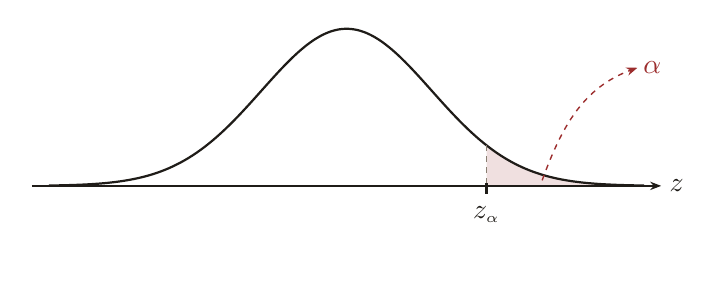
\begin{tikzpicture}[
  x=1.08cm,
  y=5cm,
  every node/.style={font=\normalsize, journalink},
  axis/.style={journalink, line width=0.8pt, -{Stealth[length=4pt]}},
  tick/.style={journalink, line width=0.8pt},
  curve/.style={journalink, line width=0.8pt},
  guide/.style={journalmuted, line width=0.5pt, dash pattern=on 2pt off 2pt},
  region/.style={journalaccent, fill opacity=0.15},
  pointer/.style={journalaccent, line width=0.5pt,
                  dash pattern=on 2pt off 2pt, -{Stealth[length=4pt]}}
]
  % ---- left edge, right edge and floor, shared with Fig. 4.4 ------------
  \path ([yshift=-1.10cm]-3.75,0) -- ([yshift=-1.10cm]4.10,0);

  % ---- the right tail block --------------------------------------------
  % Spec 1.6: from the foot of the boundary along the axis to the right end
  % of the curve, up to the curve, back along the curve, cycle.
  \fill[region]
    (1.645,0) -- (3.5,0) -- (3.5,0.0008727)
    -- plot[domain=3.5:1.645, samples=300, smooth] (\x,{\normaldensity{\x}})
    -- cycle;

  % ---- density curve ---------------------------------------------------
  \draw[curve] plot[domain=-3.5:3.5, samples=300, smooth]
    (\x,{\normaldensity{\x}});

  % ---- the boundary ----------------------------------------------------
  \draw[guide] (1.645,0.1031108) -- (1.645,0);
  \draw[tick] ([yshift=0.035cm]1.645,0) -- ([yshift=-0.106cm]1.645,0);
  \node[anchor=north, inner sep=0pt] at ([yshift=-0.25cm]1.645,0)
    {$z_{\sssig \alpha}$};

  % ---- x axis ----------------------------------------------------------
  \draw[axis] (-3.7,0) -- (3.7,0);
  \node[anchor=west, inner sep=2.8pt] at (3.7,0) {$z$};

  % ---- the area of the block, named at the head of the arrow -----------
  \draw[pointer] (2.3,0.0141) to[out=70, in=200] (3.42,0.30);
  \node[journalaccent, anchor=west, inner sep=2pt] at (3.42,0.30) {$\alpha$};

\end{tikzpicture}
\end{document}
